The theory of spatial dynamics states that the power production from individual turbine can be quite different even though they are physically located in one farm and quite close to each other. The difference might arise from wake effect , terrain condition and other environmental effects. 
To capture this relation, a spatial dynamics approach has been considered. Specifically, spatial Markov chain model \cite{rey2001spatial,carle1997modeling}. In this section, a finite state spatial dynamics model is presented that is used to derive the transition matrix for the wind turbines in a wind farm. 
A Markov chain has a series of states $n$ which are mutually exclusive of each other thus applicable to discrete data-set. A transition matrix has transition probabilities from one state to another. The fig. \ref{fig:queen} presents the spacial relationship between wind turbines. The location information is presented in the table \ref{tbl:spatial}. The polygons are created using the GeoDa \cite{anselin2006geoda} program. 

\begin{figure}
\centering
\begin{subfigure}{.5\textwidth}
  \centering
  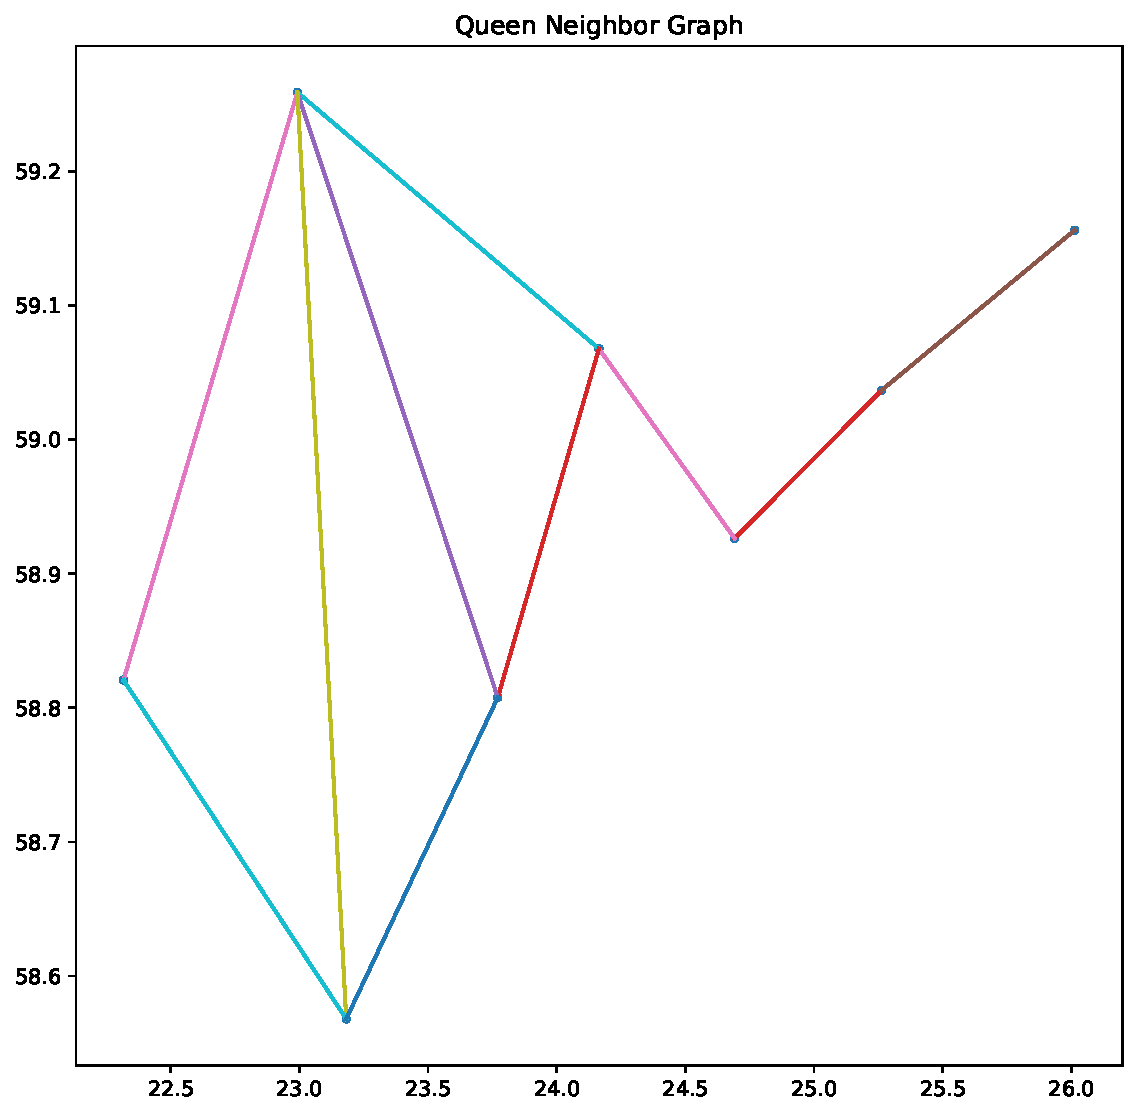
\includegraphics[width=\linewidth]{./sec/fig/queenrelationships.pdf}
 % \caption{A subfigure}
  \label{fig:sub1}
\end{subfigure}%
\begin{subfigure}{.5\textwidth}
  \centering
  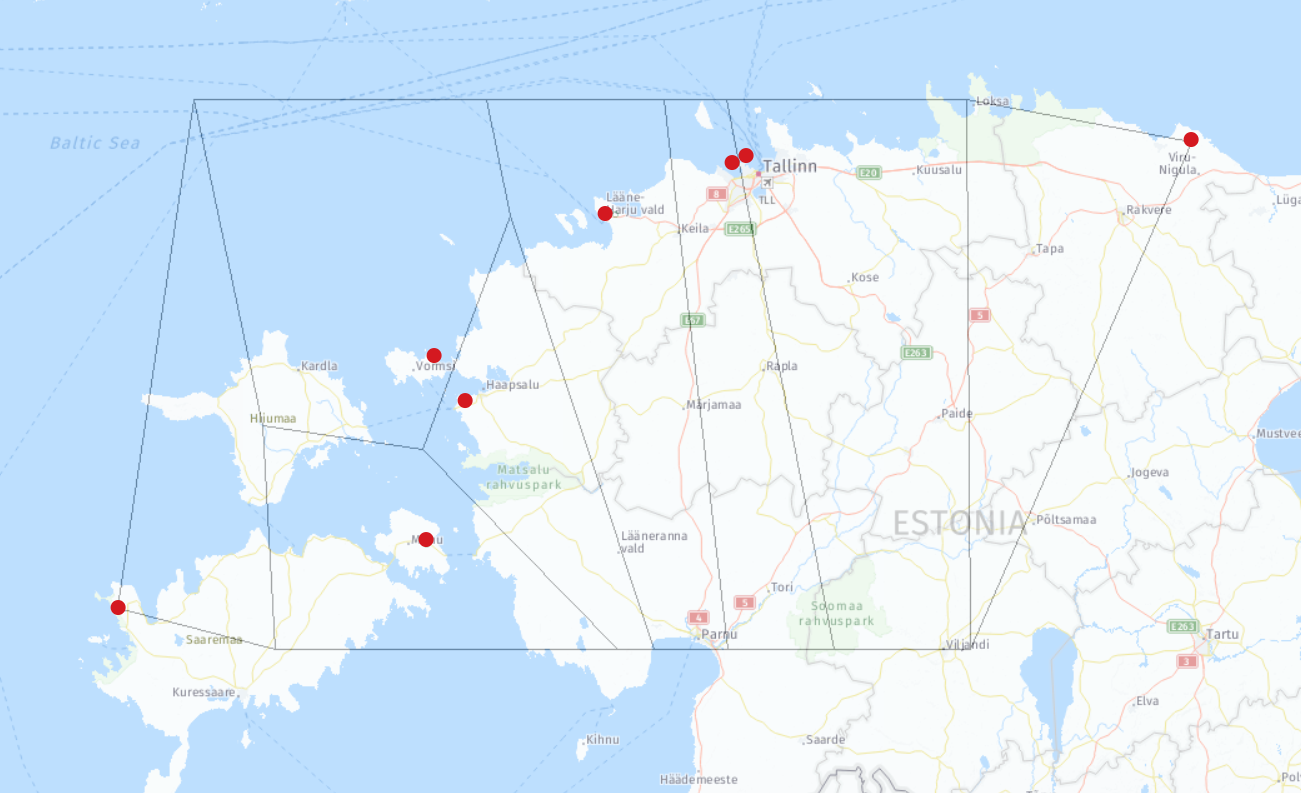
\includegraphics[width=\linewidth]{./sec/fig/thiessen_polygons.png}
 % \caption{A subfigure}
  \label{fig:sub2}
\end{subfigure}
\caption{Spatial relation between wind turbine locations: on left queens neighbor graph and on right the actual locations in Estonia}
\label{fig:queen}
\end{figure}


\begin{table}[!htbp]
\centering
\begin{tabular}{cccl} \hline
Wind turbine & Longitude		& Lattitude & Location\\ \hline
01	&	59.4784	&		24.6923	&	Paljassaare conservation area,Tallinn				\\
02	&	59.4646	&		24.6567	&	Kopli peninsula,Tallinn				\\
03	&	59.3416	&		24.1315	&	Paldiski, Harju county				\\
04	&	59.0257	&		23.3329	&	Norrby, Lääne county				\\
05	&	58.4434	&		21.9644	&	Kõruse, Saare county				\\
06	&	58.9245	&		23.4778	&	Rohuküla, Lääne county				\\
07	&	59.4953	&		26.6583	&	Iila, Lääne-Viru county				\\
08	&	58.5955	&		23.2965	&	Mõega, Saare county				\\ \hline
\end{tabular}
\caption{Location of wind turbines}
\label{tbl:spatial}
\end{table}

%\begin{itemize}
%\item why use spatial markov? pysal package
%\item Spatial and Lisa Markov description with references
%\item Location and queen plots
%\item results through tables or figures
%\end{itemize}


\subsection{Markov process}
A deterministic Markov chain has the following property

\begin{equation} \label{eq:m1}
P(X_{n+1}^t) \in A | X_0^t \ldots = x_n ) = P ( X^t_{n+1} \in A | X_n^t = x_n )
\end{equation}

In \ref{eq:m1} the Markov property of the future state $n+1$ depends only on the current state $n$ not the past state $n-1$. The process spread over all time $t_0 \leq t_1 \leq \ldots t_n \leq t_{n+1}$ and state space $x_0, \ldots x_n$. The transition kernel for the probability matrix can be expressed as in \ref{eq:m2}.

\begin{equation} \label{eq:m2}
P_{s,t} (x,A) := P(x_t \in A | X_s =x)
\end{equation}

The kernel generates transition probability value $A$ that the process takes at time $t$ given that at time $s$ the value was $x$. The transition matrix is expressed as $P(p(x,y))_{x,y \in s}$. The initial state is $P(X_0 =x)_{x \in s}$. The distribution at time $t=1$ is presented in \eqref{eq:m3}. One step transition probability is expressed in \eqref{eq:m4}. 

 \begin{align} 
P(X_1 =x) &= \sum_{x_0 \in S} P(X_0 = x_0) * P(X_1 =x | X_0 =x_0)  \\  \label{eq:m3}
p(x,y) & := P(X_{n+1} = y | X_n =x)   \\ \label{eq:m4}
\end{align}
  
